\documentclass[tikz,border=4pt]{standalone}
\usepackage{amsmath}
\usepackage{tikz}
\usetikzlibrary{arrows.meta}
\begin{document}
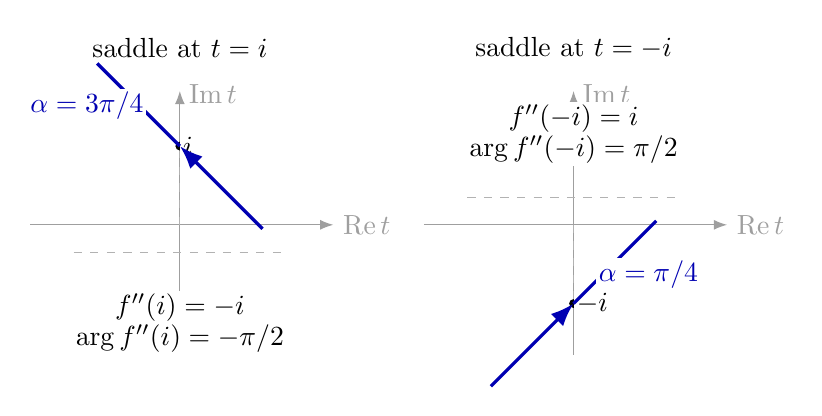
\begin{tikzpicture}[>=Latex,scale=1.0]
  \tikzset{
    axis/.style={->,gray!75},
    path/.style={very thick,blue!70!black},
    guide/.style={dashed,gray!60},
    tag/.style={fill=white,inner sep=1pt}
  }

  \begin{scope}
    \node at (0,2.25) {saddle at $t=i$};
    \draw[axis] (-1.9,0) -- (1.95,0) node[right] {$\operatorname{Re}t$};
    \draw[axis] (0,-1.65) -- (0,1.7);
    \node[tag,text=gray!75] at (0.42,1.66) {$\operatorname{Im}t$};
    \draw[guide] (-1.35,-0.35) -- (1.35,-0.35);
    \draw[guide] (0,0) -- (0,1);
    \fill (0,1) circle (1.6pt) node[tag,right] {$i$};
    \draw[path,->] (1.05,-0.05) -- (0,1);
    \draw[path] (0,1) -- (-1.05,2.05);
    \node[tag,text=blue!70!black] at (-1.18,1.52)
      {$\alpha=3\pi/4$};
    \node[align=center,tag] at (0,-1.25)
      {$f''(i)=-i$\\[-1pt]$\arg f''(i)=-\pi/2$};
  \end{scope}

  \begin{scope}[xshift=5.0cm]
    \node at (0,2.25) {saddle at $t=-i$};
    \draw[axis] (-1.9,0) -- (1.95,0) node[right] {$\operatorname{Re}t$};
    \draw[axis] (0,-1.65) -- (0,1.7);
    \node[tag,text=gray!75] at (0.42,1.66) {$\operatorname{Im}t$};
    \draw[guide] (-1.35,0.35) -- (1.35,0.35);
    \draw[guide] (0,0) -- (0,-1);
    \fill (0,-1) circle (1.6pt) node[tag,right] {$-i$};
    \draw[path,->] (-1.05,-2.05) -- (0,-1);
    \draw[path] (0,-1) -- (1.05,0.05);
    \node[tag,text=blue!70!black] at (0.95,-0.63)
      {$\alpha=\pi/4$};
    \node[align=center,tag] at (0,1.15)
      {$f''(-i)=i$\\[-1pt]$\arg f''(-i)=\pi/2$};
  \end{scope}
\end{tikzpicture}
\end{document}
